\documentclass[a4paper,12pt]{article} 
\usepackage[T2A]{fontenc}			
\usepackage[utf8]{inputenc}			
\usepackage[english,russian]{babel}	
\usepackage{amsmath,amsfonts,amssymb,amsthm,mathrsfs,mathtools} 
\usepackage{cancel}
\usepackage{multirow}
\usepackage[colorlinks, linkcolor = blue]{hyperref}
\usepackage{upgreek}\usepackage[left=2cm,right=2cm,top=2cm,bottom=3cm,bindingoffset=0cm]{geometry}
\usepackage{tikz}
\usepackage{graphicx}
\usepackage{subfig}
\usepackage{titletoc}
\usepackage{pgfplots}
\usepackage{xcolor}
\usepackage{wrapfig}
\author{Дорогинин Д.В.\\
Группа Б02-825}
\title{4.5.2. Интерференция лазерного излучения}
\date{}

%\begin{wrapfigure}{r}{0.5\textwidth}
%\begin{center}
%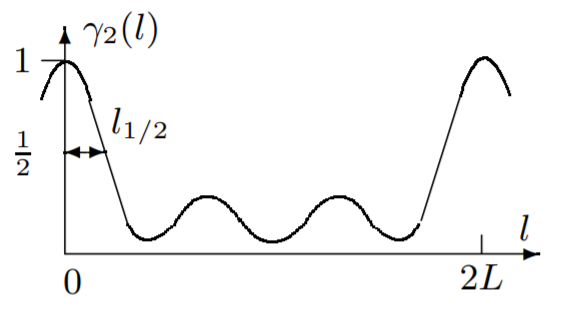
\includegraphics[width = 0.4\textwidth]{1.png}
%\end{center}
%\caption{}
%\end{wrapfigure}

%\begin{wrapfigure}{r}{0.5\textwidth}
%\begin{center}
%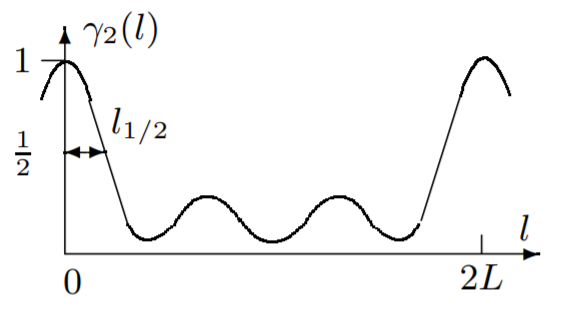
\includegraphics[width = 0.4\textwidth]{1.png}
%\end{center}
%\caption{}
%\end{wrapfigure}

\begin{document}
\maketitle
\textbf{Цель работы}: исследовать зависимость видности интерфереционной картины от разности хода интерферирующих лучей и от их поляризации.


\textbf{В работе используются}: He-Ne лазер, интерферометр Майкельсона с подвижным зеркалом, фотодиод с усилителем, осциллограф С1-76, поляроид, линейка.
\section*{Теория}
\subsection*{Гелий-неоновый лазер}
Лазер представляет собой интерферометр Фабри-Перо -- газовую трубку с двумя параллельными зеркалами по обе стороны. В лазере длиной $L$ для излучения вдоль оси для резонансных частот выполняется
\begin{equation}
f_m = \dfrac{c}{\lambda_m} = \dfrac{mc}{2L}.
\end{equation}
Условие генерации может выполняться для сразу нескольких колебаний с частостами $f_m$, разположенными в диапазоне генерации $2\Delta F$. В этом случае генерируется несколько волн -- \textit{мод} -- межмодовое расстояние для которых
\begin{equation}
\Delta \nu = f_{m+1} - f_m = \dfrac{c}{2L}.
\end{equation}
Число мод можно оценить как 
\begin{equation}
N \approx 1 + \dfrac{2\Delta F}{\Delta \nu}.
\end{equation}
\subsection*{Видимость}
Видимость интерфереционной картины -- параметр, определяемый формулой
\begin{equation}
\gamma = \dfrac{I_{max} - I_{min}}{I_{max} + I_{min}},
\end{equation}
где $I_{max}$, $I_{min}$ -- максимальная и минимальная интенсивности света интерфереционной картины вблизи выбранной точки. Разобьём его на произведение функций параметров установки
$$
\gamma = \gamma_1 \gamma_2 \gamma_3.
$$
Здесь $\gamma_1$ отвечает за соотношение интенсивности интерферирующих волн:
\begin{equation}
\gamma_1 = \dfrac{2\sqrt{\delta}}{1+\delta},
\end{equation}
где $\delta = \frac{B_m^2}{A_m^2}$, $A_m$ и $B_m$ -- амплитуды волн. Параметр $\delta$ определяется устройством разделения волн.\\
Функция $\gamma_2$ отвечает за влияние разности хода и спектрального состава волн,
\begin{wrapfigure}{r}{0.4\textwidth}
\begin{center}
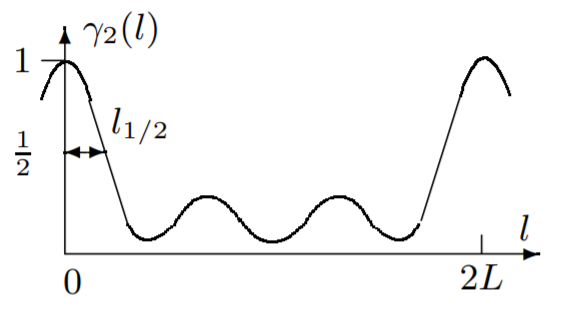
\includegraphics[width = 0.4\textwidth]{1.png}
\vspace{-20pt}
\end{center}
\caption{Зависимость $\gamma_2 = \gamma_2(l)$.}
\end{wrapfigure}
$$
\gamma_2 = \dfrac{\sum\limits_n A^2_n \cos \frac{2\pi \Delta \nu n l}{c}}{\sum\limits_n A_n^2},
$$
где $l$ -- разность хода, $\Delta \nu$ -- спектральный состав излучения, $A_n^2$ -- интенсивности мод. В непрерывном пределе получим
$$
\gamma_2 = e^{-\left(\frac{\pi \Delta F l}{c}\right)^2}
$$
-- для гауссова линии излучения с полушириной $\Delta F$ получили гауссову зависимость $\gamma_2 = \gamma_2(l)$ с полушириной 
\begin{equation}
l_{1/2} = \dfrac{c}{\pi \Delta F}\sqrt{\ln 2} \approx \dfrac{0.26 c}{\Delta F}.
\end{equation}
Последняя функция $\gamma_3$ отвечает за разность в поляризации. Если $\alpha$ -- угол между плоскостями поляризаций волн, то
\begin{equation}
\gamma_3 = |\cos \alpha|.
\end{equation}
\subsection*{Установка}
\begin{figure}[h]
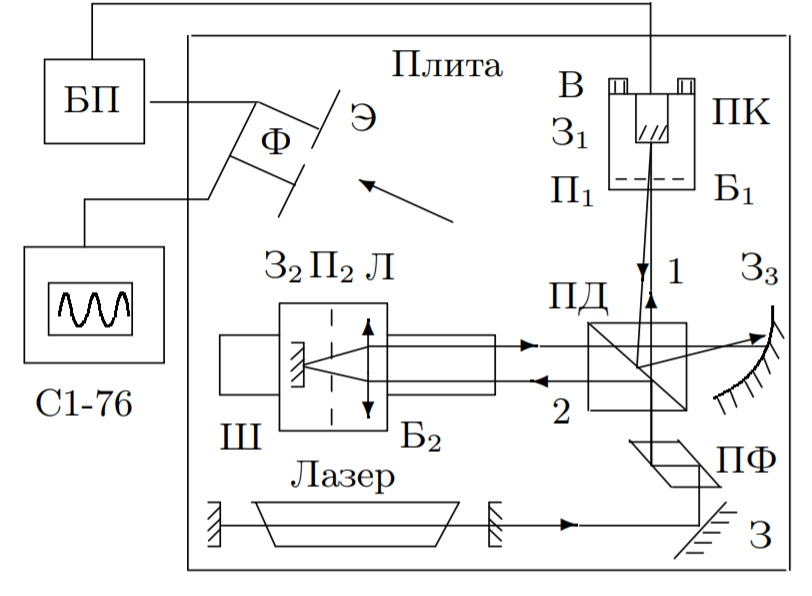
\includegraphics[scale=0.55]{2.png}
\centering
\caption{Схема установки.}
\end{figure}
В работе используется интерферометр Майкельсона (Рис. 2). Луч лазера, отражённый от зеркала З и прошедший через параллелепипед Френеля (ПФ), делится делительной призмой ДП на два луча. Первый проходит блок $\text{Б}_1$ с поляроидом $\text{П}_1$ и зеркалом $\text{З}_1$, прикленным к пьезокерамике, которая может совершать малые колебания вдоль луча, с возможность изменения угла наклона зеркала. Второй проходит блок $\text{Б}_2$ с линзой Л, поляроидом $\text{П}_2$ и зеркалом $\text{З}_2$ в фокальной плоскости линзы, чтобы выходящий луч, в отличие от первого, был параллелен входящему. Оба луча, проходя ДП, попадают на сферическое зеркало $\text{З}_3$ и интерферируют на экране. Интенсивность света считывается фотодиодом на осциллограф через щель, параллельную интерфереционным полосам, в центре экрана. На экране осциллографа наблюдаются колебания с изменяющимся периодом, так как на пьезокерамику подаются напряжение, из-за чего её длина колеблется.
\begin{wrapfigure}{l}{0.4\textwidth}
\begin{center}
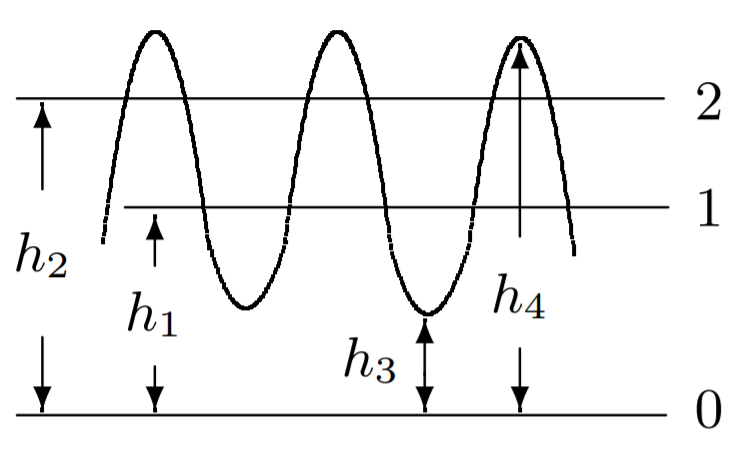
\includegraphics[width = 0.4\textwidth]{3.png}
\vspace{-40pt}
\end{center}
\caption{Осциллограмма сигналов фотодиода.}
\end{wrapfigure}
По картине на экране осциллографа можно определить параметры видимости по следующим формулам:
\begin{equation}
\delta = \dfrac{h_1}{h_2},
\end{equation}
\begin{equation}
\gamma = \dfrac{h_4 - h_3}{h_4 + h_3},
\end{equation}
Здесь 0 -- уровень при отсутствии лучей, 1 и 2 -- при закрытии одного из них. Используя $\delta$, можно рассчитать $\gamma_1$ по формуле (5).\\ 
При условии одинаковой поляризации лучей ($\alpha = 0$),
\begin{equation}
\gamma_2 = \dfrac{\gamma}{\gamma_1}.
\end{equation}
Если же разность хода отсутствует ($l = 0$), то
\begin{equation}
\gamma_3 = \dfrac{\gamma}{\gamma_1}.
\end{equation}
\section*{Ход работы}
Пронаблюдаем интерференционную картину на экране. Поставим дополнительный поляроид между лазером и ПФ, вращая его, наблюдаем, что поляризация линейная. Перенесём поляроид и поставим его на пути луча, выходящего из ПФ. Наблюдаем, что теперь у луча круговая поляризация. Установим минимальную чёткость интерфереционной картину вращением $\text{П}_1$. Внесём дополнительный поляроид на пути луча, идущего на экран, -- интерфереционная картина вновь возникает из-за поляризованности света, так как после прохождения второго поляроида два луча будут иметь одну поляризацию, задаваемую поляроидом.\\
Исследуем зависимость видности интерфереционной картина от угла $\alpha$ между плоскостями поляризации интерферирущих лучей. В нашем случае $\alpha$ -- угол поворота поляроида $\text{П}_1$. Результаты измерений представлены в Таблице 1. При подсчётах были использованы формулы (8), (5), (9) и (11). Погрешность измерения угла приборная $\sigma_\alpha = 1^\circ$, погрешность измерения всех $h$ -- половина цены деления $\sigma_{h_i} = 0.1 \text{ дел}$. Для $\gamma_3$ погрешность вычисляется по формуле 
$$
\sigma_{\gamma_3} = \sqrt{\sum\limits_{i=1}^4\left(\dfrac{\partial \gamma_3}{\partial h_i}\right)^2 \sigma^2_{h_i}}.
$$
Представим результаты на графике $\gamma_3 = \gamma_3(\cos \alpha)$ (Рис. 4), убеждаемся в верности теоретической зависимости (7). На графике для $\alpha = 0$ значение $\gamma_3$ было принято за 1, а все остальные $\gamma_3$ поделены на полученное для $\alpha = 0$, чтобы исключить влияние $\gamma_2$ на результат.
\newpage
\begin{table}[h]
\begin{tabular}{|c|c|c|c|c|c|c|}
\hline
$\alpha$ & $h_1$, дел & $h_2$, дел & $h_3$, дел & $h_4$, дел & $\gamma_3$ & $\sigma_{\gamma_3}$ \\ \hline
0        & 2.6        & 1.8        & 0.6        & 3.8        & 0.74       & 0.18      \\ \hline
10       & 2.8        & 1.5        & 0.6        & 3.7        & 0.76       & 0.18      \\ \hline
20       & 3.0        & 1.6        & 0.8        & 3.9        & 0.69       & 0.18      \\ \hline
30       & 3.0        & 1.5        & 0.9        & 3.6        & 0.64       & 0.18      \\ \hline
40       & 2.4        & 1.4        & 0.8        & 3.0        & 0.60       & 0.17      \\ \hline
50       & 2.0        & 1.4        & 0.8        & 2.6        & 0.54       & 0.16      \\ \hline
60       & 1.2        & 1.4        & 0.8        & 1.8        & 0.39       & 0.15      \\ \hline
70       & 0.6        & 1.2        & 0.8        & 1.3        & 0.25       & 0.15      \\ \hline
80       & 1.1        & 3.1        & 3.8        & 4.8        & 0.13       & 0.16      \\ \hline
90       & 1.0        & 3.0        & 3.6        & 4.2        & 0.09       & 0.16      \\ \hline
100      & 1.2       & 3.0        & 3.0          & 4.2        & 0.18       & 0.16      \\ \hline
110      & 1.7        & 2.7        & 1.2        & 2.0        & 0.26       & 0.15      \\ \hline
120      & 2.6        & 2.8        & 1.5        & 2.8        & 0.30       & 0.15      \\ \hline
130      & 3.4        & 2.8        & 1.7        & 3.4        & 0.33       & 0.15      \\ \hline
140      & 3.2        & 2.8        & 1.4        & 3.4        & 0.42       & 0.15      \\ \hline
\end{tabular}
\centering
\caption{Результаты измерений для $\gamma_3 = \gamma_3(\alpha)$.}
\end{table} 

\begin{figure}[h]
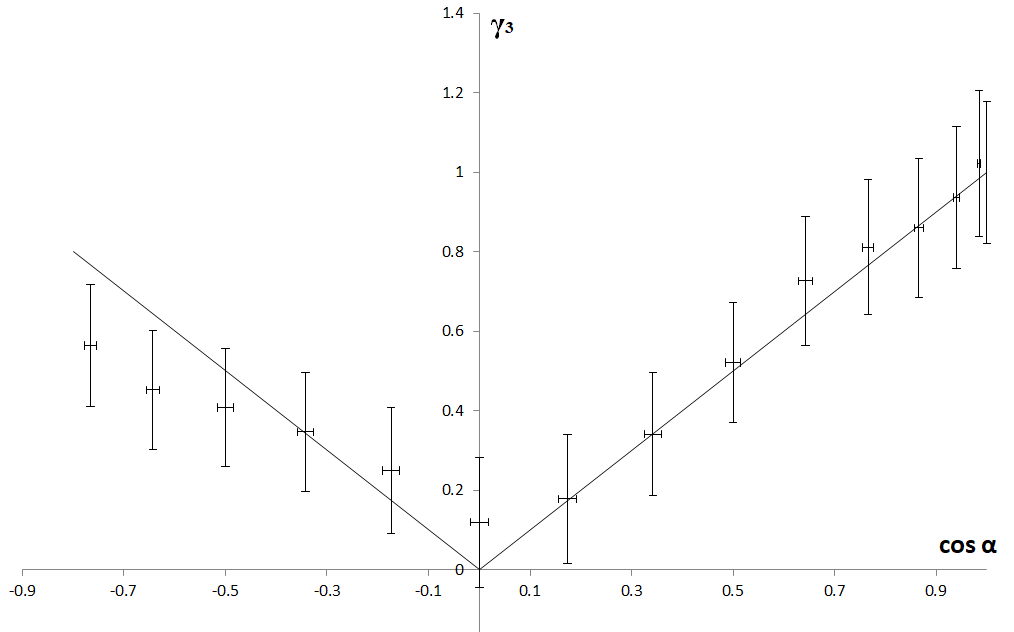
\includegraphics[scale=0.6]{4.png}
\centering
\caption{Зависимость $\gamma_3 = \gamma_3(\cos \alpha)$.}
\end{figure}
Теперь исследуем зависимость видимости интерфереционной картины от разности хода между лучами. Для этого будем перемещать блок $\text{Б}_2$ вдоль направления распространения луча, координата блока $x$ будет определять разность хода. Значения измерений представлены в Таблице 2, а так же на графике (Рис. 5).\\
На графике явно видны два максимума -- на $x_1 = 14\pm 2 \text{ см}$ и на $x_2 = 76 \pm 2 \text{ см}$. Тогда $L = \frac{1}{2}(x_2 - x_1) = 31.0 \pm 1.4 \text{ см}$. Отсюда из формулы (2)
$$
\Delta \nu = \dfrac{c}{2L} = (48 \pm 2) \cdot 10^7 \text{ Гц}.
$$
Погрешность считается из соотношения $\varepsilon_{\Delta\nu} = \varepsilon_{L}$. Полуширина кривой из графика
$$
l_{1/2} \approx 10 \pm 2 \text{ см},
$$
откуда по формуле (6)
$$
\Delta F = \dfrac{0.26 c}{l_{1/2}} = (78 \pm 16) \cdot 10^7 \text{ Гц}.
$$
Погрешность считается аналогично $\Delta \nu$. Тогда по формуле (3) число мод
$$
N = 1 + \dfrac{2\Delta F}{\Delta \nu} = 4 \pm 1, 
$$
погрешность рассчитана по формуле 
$$
\sigma_N = \sqrt{\left( \dfrac{\partial N}{\partial \Delta F} \right)^2 \sigma^2_{\Delta F} + \left( \dfrac{\partial N}{\partial \Delta \nu} \right)^2 \sigma^2_{\Delta \nu}}
$$
с округлением до целых.
\begin{figure}[h]
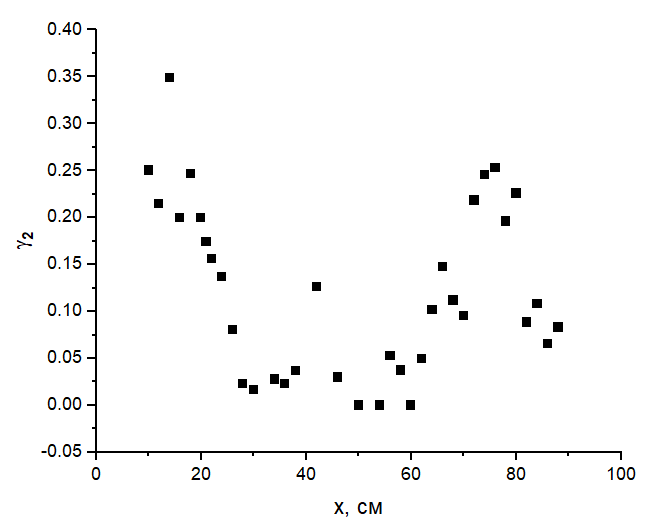
\includegraphics[scale=0.8]{5.png}
\centering
\caption{Зависимость $\gamma_2 = \gamma_2(x)$.}
\end{figure}
\begin{table}[h]
\begin{tabular}{|c|c|c|c|c|c|}
\hline
$x$, см & $h_1$, дел & $h_2$, дел & $h_3$, дел & $h_4$, дел & $\gamma_2$ \\ \hline
10      & 2.2        & 2.4        & 2.4        & 4.0        & 0.25       \\ \hline
12      & 2.3        & 0.8        & 2.6        & 3.8        & 0.21       \\ \hline
14      & 2.2        & 1.2        & 2.3        & 4.6        & 0.35       \\ \hline
16      & 2.2        & 3.2        & 4.7        & 7.0        & 0.20       \\ \hline
18      & 2.2        & 1.2        & 2.6        & 4.2        & 0.25       \\ \hline
20      & 2.2        & 2.2        & 3.6        & 5.4        & 0.20       \\ \hline
21      & 2.2        & 2.2        & 3.8        & 5.4        & 0.17       \\ \hline
22      & 2.2        & 2.2        & 3.8        & 5.2        & 0.16       \\ \hline
24      & 2.2        & 2.0        & 3.8        & 5.0        & 0.14       \\ \hline
26      & 2.2        & 3.9        & 4.8        & 5.6        & 0.08       \\ \hline
28      & 2.2        & 2.0        & 4.2        & 4.4        & 0.02       \\ \hline
30      & 2.2        & 1.0        & 3.2        & 3.3        & 0.02       \\ \hline
34      & 2.2        & 1.4        & 3.6        & 3.8        & 0.03       \\ \hline
36      & 2.2        & 2.0        & 4.2        & 4.4        & 0.02       \\ \hline
38      & 2.2        & 0.8        & 3.0        & 3.2        & 0.04       \\ \hline
42      & 2.2        & 0.6        & 2.6        & 3.2        & 0.13       \\ \hline
46      & 2.2        & 1.2        & 3.4        & 3.6        & 0.03       \\ \hline
50      & 2.2        & 0.8        & 3.0        & 3.0        & 0.00       \\ \hline
54      & 2.4        & 0.2        & 2.4        & 2.4        & 0.00       \\ \hline
56      & 2.4        & 0.4        & 2.6        & 2.8        & 0.05       \\ \hline
58      & 2.4        & 0.8        & 3.0        & 3.2        & 0.04       \\ \hline
60      & 2.4        & 0.6        & 3.0        & 3.0        & 0.00       \\ \hline
62      & 2.4        & 0.4        & 2.8        & 3.0        & 0.05       \\ \hline
64      & 2.4        & 0.4        & 2.6        & 3.0        & 0.10       \\ \hline
66      & 2.4        & 0.4        & 2.6        & 3.2        & 0.15       \\ \hline
68      & 2.4        & 0.8        & 2.8        & 3.4        & 0.11       \\ \hline
70      & 2.4        & 0.4        & 2.8        & 3.2        & 0.10       \\ \hline
72      & 2.4        & 0.6        & 2.6        & 3.7        & 0.22       \\ \hline
74      & 2.4        & 0.8        & 2.6        & 4.0        & 0.24       \\ \hline
76      & 2.5        & 1.0        & 2.7        & 4.3        & 0.25       \\ \hline
78      & 2.8        & 1.2        & 3.2        & 4.6        & 0.20       \\ \hline
80      & 2.4        & 2.4        & 3.6        & 5.7        & 0.23       \\ \hline
82      & 3.2        & 1.6        & 4.4        & 5.2        & 0.09       \\ \hline
84      & 3.4        & 1.0        & 4.0        & 4.8        & 0.11       \\ \hline
86      & 3.4        & 1.6        & 4.6        & 5.2        & 0.07       \\ \hline
88      & 3.4        & 2.2        & 3.4        & 4.0        & 0.08       \\ \hline
\end{tabular}
\centering
\caption{Результаты измерений для $\gamma_2 = \gamma_2(x)$.}
\end{table}
\end{document}